% Template for PLoS
% Version 3.5 March 2018
%
% % % % % % % % % % % % % % % % % % % % % %
%
% -- IMPORTANT NOTE
%
% This template contains comments intended
% to minimize problems and delays during our production
% process. Please follow the template instructions
% whenever possible.
%
% % % % % % % % % % % % % % % % % % % % % % %
%
% Once your paper is accepted for publication,
% PLEASE REMOVE ALL TRACKED CHANGES in this file
% and leave only the final text of your manuscript.
% PLOS recommends the use of latexdiff to track changes during review, as this will help to maintain a clean tex file.
% Visit https://www.ctan.org/pkg/latexdiff?lang=en for info or contact us at latex@plos.org.
%
%
% There are no restrictions on package use within the LaTeX files except that
% no packages listed in the template may be deleted.
%
% Please do not include colors or graphics in the text.
%
% The manuscript LaTeX source should be contained within a single file (do not use \input, \externaldocument, or similar commands).
%
% % % % % % % % % % % % % % % % % % % % % % %
%
% -- FIGURES AND TABLES
%
% Please include tables/figure captions directly after the paragraph where they are first cited in the text.
%
% DO NOT INCLUDE GRAPHICS IN YOUR MANUSCRIPT
% - Figures should be uploaded separately from your manuscript file.
% - Figures generated using LaTeX should be extracted and removed from the PDF before submission.
% - Figures containing multiple panels/subfigures must be combined into one image file before submission.
% For figure citations, please use "Fig" instead of "Figure".
% See http://journals.plos.org/plosone/s/figures for PLOS figure guidelines.
%
% Tables should be cell-based and may not contain:
% - spacing/line breaks within cells to alter layout or alignment
% - do not nest tabular environments (no tabular environments within tabular environments)
% - no graphics or colored text (cell background color/shading OK)
% See http://journals.plos.org/plosone/s/tables for table guidelines.
%
% For tables that exceed the width of the text column, use the adjustwidth environment as illustrated in the example table in text below.
%
% % % % % % % % % % % % % % % % % % % % % % % %
%
% -- EQUATIONS, MATH SYMBOLS, SUBSCRIPTS, AND SUPERSCRIPTS
%
% IMPORTANT
% Below are a few tips to help format your equations and other special characters according to our specifications. For more tips to help reduce the possibility of formatting errors during conversion, please see our LaTeX guidelines at http://journals.plos.org/plosone/s/latex
%
% For inline equations, please be sure to include all portions of an equation in the math environment.
%
% Do not include text that is not math in the math environment.
%
% Please add line breaks to long display equations when possible in order to fit size of the column.
%
% For inline equations, please do not include punctuation (commas, etc) within the math environment unless this is part of the equation.
%
% When adding superscript or subscripts outside of brackets/braces, please group using {}.
%
% Do not use \cal for caligraphic font.  Instead, use \mathcal{}
%
% % % % % % % % % % % % % % % % % % % % % % % %
%
% Please contact latex@plos.org with any questions.
%
% % % % % % % % % % % % % % % % % % % % % % % %

\documentclass[10pt,letterpaper]{article}
\usepackage[top=0.85in,left=2.75in,footskip=0.75in]{geometry}

% amsmath and amssymb packages, useful for mathematical formulas and symbols
\usepackage{amsmath,amssymb}

% Use adjustwidth environment to exceed column width (see example table in text)
\usepackage{changepage}

% Use Unicode characters when possible
\usepackage[utf8x]{inputenc}

% textcomp package and marvosym package for additional characters
\usepackage{textcomp,marvosym}

% cite package, to clean up citations in the main text. Do not remove.
% \usepackage{cite}

% Use nameref to cite supporting information files (see Supporting Information section for more info)
\usepackage{nameref,hyperref}

% line numbers
\usepackage[right]{lineno}

% ligatures disabled
\usepackage{microtype}
\DisableLigatures[f]{encoding = *, family = * }

% color can be used to apply background shading to table cells only
\usepackage[table]{xcolor}

% array package and thick rules for tables
\usepackage{array}

% create "+" rule type for thick vertical lines
\newcolumntype{+}{!{\vrule width 2pt}}

% create \thickcline for thick horizontal lines of variable length
\newlength\savedwidth
\newcommand\thickcline[1]{%
  \noalign{\global\savedwidth\arrayrulewidth\global\arrayrulewidth 2pt}%
  \cline{#1}%
  \noalign{\vskip\arrayrulewidth}%
  \noalign{\global\arrayrulewidth\savedwidth}%
}

% \thickhline command for thick horizontal lines that span the table
\newcommand\thickhline{\noalign{\global\savedwidth\arrayrulewidth\global\arrayrulewidth 2pt}%
\hline
\noalign{\global\arrayrulewidth\savedwidth}}


% Remove comment for double spacing
%\usepackage{setspace}
%\doublespacing

% Text layout
\raggedright
\setlength{\parindent}{0.5cm}
\textwidth 5.25in
\textheight 8.75in

% Bold the 'Figure #' in the caption and separate it from the title/caption with a period
% Captions will be left justified
\usepackage[aboveskip=1pt,labelfont=bf,labelsep=period,justification=raggedright,singlelinecheck=off]{caption}
\renewcommand{\figurename}{Fig}

% Use the PLoS provided BiBTeX style
% \bibliographystyle{plos2015}

% Remove brackets from numbering in List of References
\makeatletter
\renewcommand{\@biblabel}[1]{\quad#1.}
\makeatother



% Header and Footer with logo
\usepackage{lastpage,fancyhdr,graphicx}
\usepackage{epstopdf}
%\pagestyle{myheadings}
\pagestyle{fancy}
\fancyhf{}
%\setlength{\headheight}{27.023pt}
%\lhead{
\includegraphics[width=2.0in]{PLOS-submission.eps}}
\rfoot{\thepage/\pageref{LastPage}}
\renewcommand{\headrulewidth}{0pt}
\renewcommand{\footrule}{\hrule height 2pt \vspace{2mm}}
\fancyheadoffset[L]{2.25in}
\fancyfootoffset[L]{2.25in}
\lfoot{\today}

%% Include all macros below

\newcommand{\lorem}{{\bf LOREM}}
\newcommand{\ipsum}{{\bf IPSUM}}





\usepackage{forarray}
\usepackage{xstring}
\newcommand{\getIndex}[2]{
  \ForEach{,}{\IfEq{#1}{\thislevelitem}{\number\thislevelcount\ExitForEach}{}}{#2}
}

\setcounter{secnumdepth}{0}

\newcommand{\getAff}[1]{
  \getIndex{#1}{}
}

\providecommand{\tightlist}{%
  \setlength{\itemsep}{0pt}\setlength{\parskip}{0pt}}

\begin{document}
\vspace*{0.2in}

% Title must be 250 characters or less.
\begin{flushleft}
{\Large
\textbf\newline{CEEDS Weather Dashboard} % Please use "sentence case" for title and headings (capitalize only the first word in a title (or heading), the first word in a subtitle (or subheading), and any proper nouns).
}
\newline
% Insert author names, affiliations and corresponding author email (do not include titles, positions, or degrees).
\\
Julia Lee\textsuperscript{},
Marta Garcia\textsuperscript{},
Mirella Hernandez\textsuperscript{}\\
\bigskip
\bigskip
\end{flushleft}
% Please keep the abstract below 300 words
\section*{Abstract}
We were tasked with finding a way to better showcase weather data from
the MacLeish field station. We were also tasked with incorporating
interactive graphics and allowing users to download and filter the data.
So we decided to use the shiny and Shiny Dashboard packages in R to
build an interactive dashboard. We also wrote a package to get the data
from the MacLeish server.

% Please keep the Author Summary between 150 and 200 words
% Use first person. PLOS ONE authors please skip this step.
% Author Summary not valid for PLOS ONE submissions.

\linenumbers

% Use "Eq" instead of "Equation" for equation citations.
\section{Introduction}\label{introduction}

\section{Methods}\label{methods}

\subsection{Shiny app:}\label{shiny-app}

To solve our problem, we had many options on how to create a better way
of displaying the weather data. We first discussed the possibility of
making a new website in HTML but we ultimately decided to build a Shiny
App using the Shiny\footnote{Winston Chang, Joe Cheng, JJ Allaire, Yihui
  Xie and Jonathan McPherson (2018). shiny: Web Application Framework
  for R. R package version 1.2.0.
  https://CRAN.R-project.org/package=shiny} and Shiny
Dashboard\footnote{Winston Chang and Barbara Borges Ribeiro (2018).
  shinydashboard: Create Dashboards with `Shiny'. R package version
  0.7.1. https://CRAN.R-project.org/package=shinydashboard} packages in
R. Shiny is a package that allows us ``to build interactive web
applications (apps) straight from R.'' Shiny allows the user to be able
better communicate data with interactive charts, visualizations, text
and tables. We then decided to use Shiny Dashboard which is a package
that allows us to create an interactive dashboard using Shiny. Because
our problem was to find a way to display interactive data
visualizations, the Shiny package seemed to be the better option because
that is what it was built to do. Shiny also allows us to make normally
static plots like ggplots interactive and take in user input so we don't
need to use HTML widgets.

Shiny is based on a reactive programming model which means that it takes
in input given by the user of the app and acts accordingly. Shiny apps
have two components: the user interface (UI) and the server. You can
think of the UI as what the user of your app will see when they open
your app. The UI component converts your code in R and generates it into
a web document in HTML. UI contains the instruction about what you want
the user to see and the layout of your app. our UI is where we define
the dashboard page. And inside this dashboard page we define our
elements like the sidebar menu, tabs, the dashboard body (Tab items,
boxes, text). The server is the R code that tells your shiny server what
to do when the user does certain things in the app. The server is a
function where we define the output and tell the host of our app what to
do with the user input. Server function is where we render the charts,
visualizations, and tables. We then knit together the Server function
and UI using the ShinyApp (UI, server) function in the Shiny package.

So we built a Shiny dashboard. Our dashboard has a sidebar menu that has
four tab items. One tab item we built was the current weather tab. The
current weather tab gives the user the the current 10 minute weather for
WhatelyMet and OrchardMet. Because we wanted to have our data be shown
as a text object and not a table, our code for this tab was largely done
using HTML. We used a bit of HTML to change the sizing of the text and
the alignment of the rows. To make the teal boxes, we used the
shinydashboard Plus package\footnote{David Granjon (2019).
  shinydashboardPlus: Add More `AdminLTE2' Components to
  `shinydashboard'. R package version 0.7.0.
  https://CRAN.R-project.org/package=shinydashboardPlus}, allowed us to
make a clear, concise first page of our Shiny app. Another tab on our
dashboard is the about tab where we explain our project and give
information about the weather stations.

\includegraphics[width=3.64583in]{Weather Dashboard.png}\footnote{Fig 2.
  Example of a what our sidebar menu and dashboard looks like}

Another tab that we built was the historic data tab. We made a way for
the user to switch between daily data for OrchardMet and WhatelyMet in
the historic data tab, this means the graphs shown are reactive and are
based on the data set that was selected by the user. We did by making a
reactive function inside the server that allows people to switch between
data sets, this function we call datasetInput. We made graphs mapping 3
(Wind speed, precipitation, temperature) variables over time. To do
build these graphs we used the highcharter package\footnote{A Wrapper
  for the `Highcharts' Library. R package version 0.7.0.
  https://CRAN.R-project.org/package=highcharter} that allows the user
to filter the data based on a certain time period and high charter also
has a feature that enables users to download the data used to make the
graphic. 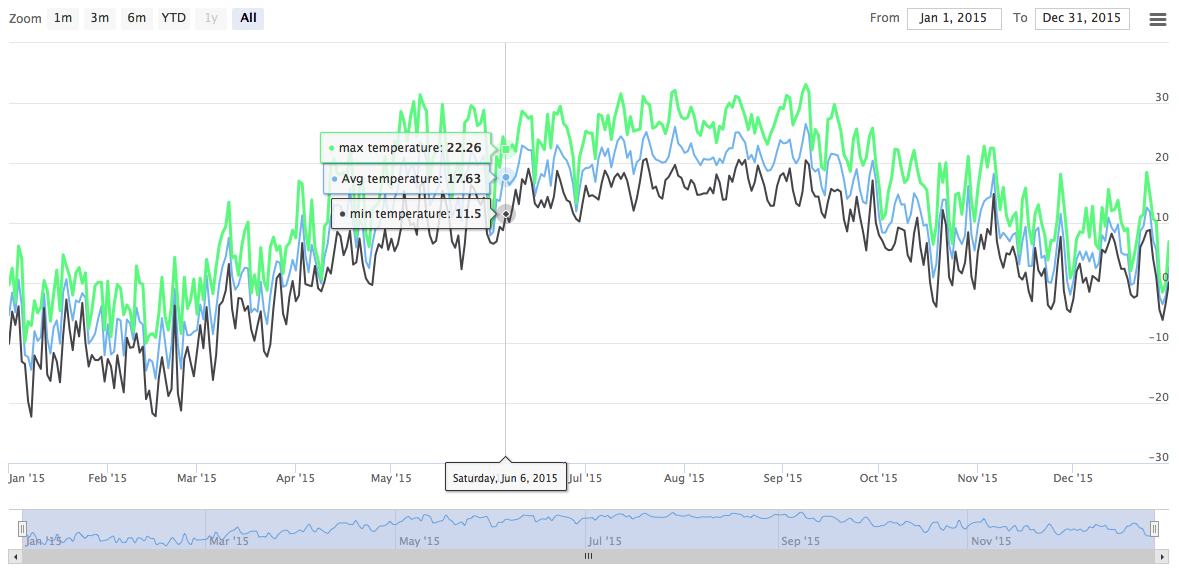
\includegraphics[width=3.64583in]{highchart.png}\footnote{Fig
  3. Example of a Highcharter graph that shows temperature}

We also made a visualization where the user can make a custom
correlation graph by picking the variables that they want. We made this
correlation scatterplot by using ggplot and ggplotly to make the graphic
more interactive. We also made a windrose graph to show wind speed and
direction using ggplot. A wind rose is a polar chart which shows the
user how wind speed and wind direction are distributed at a over a
specific period of time. We also created a way to allow the user to
choose a variable and get summary statistics on that variable. In this
tab, we made the graphs be in a fluid page, this allows for the size of
the boxes and visuals to change based on the size of the window. We then
put all of our content for the tab in separate boxes that are
collapsible. We did this to minimize users' scrolling.
\includegraphics[width=3.64583in]{windrose.png}\footnote{Fig 4. Example
  of a Windrose graph}

The last tab we made is the raw data tab. This tab allows the user to
filter the data based on columns and the user can also choose between
daily data for OrchardMet and WhatelyMet. This tab also allows the user
to search the data table using the DT package.

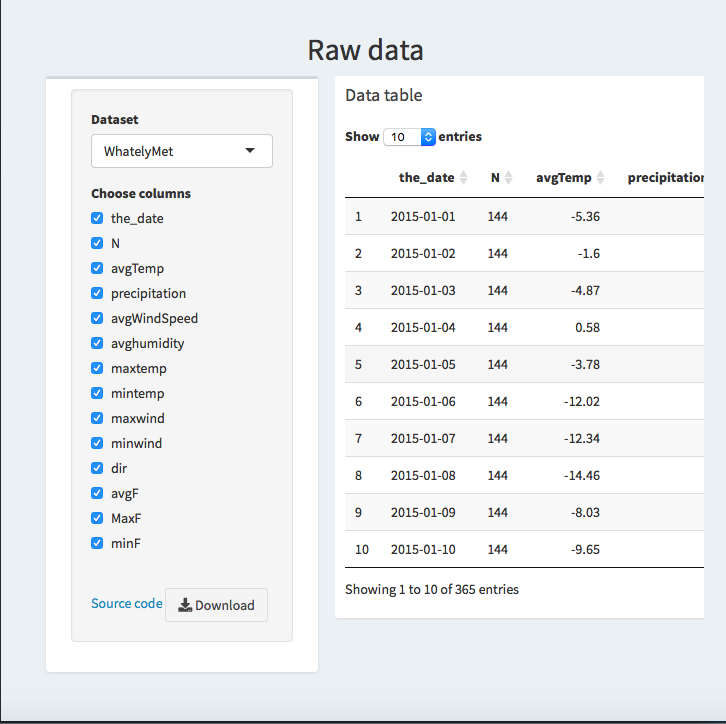
\includegraphics[width=3.64583in]{raw data tab.png}\footnote{Fig 5. A
  screenshot of our raw data tab}

\subsection{Ceeds package:}\label{ceeds-package}

The data from the two weather stations is currently being saved on the
Macleish Server hosted at Smith college. We used the Macleish
package\footnote{Benjamin S. Baumer, Rose Goueth, Wencong Li, Weijia
  Zhang and Nicholas Horton (2018). macleish: Retrieve Data from
  MacLeish Field Station. R package version 0.3.2.
  https://CRAN.R-project.org/package=macleish} to fetch the two data
tables from the server. However this involved a lot of code that would
have to be repeated anytime we wanted to run the app. So we decided to
write an R package called ``ceeds'' to more efficiently do these tasks.
This package was also built Help other students to work on the MacLeish
weather data. We wrote a function that uses the Macleish package and
fetches 2 data sets (Whately, Orchard) that is updated every ten
minutes. We also created a function,get\_daily(), inside the package
that takes a data set and gives the user the data grouped by date. Our
data from the server comes in 10 minute increments but we might want to
group by date. So we used the Lubridate package\footnote{Garrett
  Grolemund, Hadley Wickham (2011). Dates and Times Made Easy with
  lubridate. Journal of Statistical Software, 40(3), 1-25. URL
  http://www.jstatsoft.org/v40/i03/.} that was very helpful. It allowed
us to Parsed timestamps into dates (turning variables into dates that r
can recognize as such). This allowed us to group our data by date.

\section*{References}\label{references}
\addcontentsline{toc}{section}{References}

\subsection{Packages:}\label{packages}

lubridate: Garrett Grolemund, Hadley Wickham (2011). Dates and Times
Made Easy with lubridate. Journal of Statistical Software, 40(3), 1-25.
URL http://www.jstatsoft.org/v40/i03/.

highcharter: Joshua Kunst (2019). highcharter: A Wrapper for the
`Highcharts' Library. R package version 0.7.0.
https://CRAN.R-project.org/package=highcharter

macleish: Benjamin S. Baumer, Rose Goueth, Wencong Li, Weijia Zhang and
Nicholas Horton (2018). macleish: Retrieve Data from MacLeish Field
Station. R package version 0.3.2.
https://CRAN.R-project.org/package=macleish

shiny: Winston Chang, Joe Cheng, JJ Allaire, Yihui Xie and Jonathan
McPherson (2018). shiny: Web Application Framework for R. R package
version 1.2.0. https://CRAN.R-project.org/package=shiny

shinydashboard: Winston Chang and Barbara Borges Ribeiro (2018).
shinydashboard: Create Dashboards with `Shiny'. R package version 0.7.1.
https://CRAN.R-project.org/package=shinydashboard

shinydashboardPlus: David Granjon (2019). shinydashboardPlus: Add More
`AdminLTE2' Components to `shinydashboard'. R package version 0.7.0.
https://CRAN.R-project.org/package=shinydashboardPlus

\nolinenumbers


\end{document}

